%BAB_3 LAPORAN KP

\chapter{PERANCANGAN SISTEM}
Pada bab ini akan disajikan mekanisme perancangan alat, baik perangkat keras ataupun perangkat lunak untuk mewujudkan sebuah robot lengan. Tahapan perancangan dimulai dari perancangan diagram blok sistem, perancangan perangkat keras, perancangan perangat lunak, perancangan kinematika balik, dan integrasi keseluruhan program. 
\section{ Diagram Blok Sistem }
Secara garis besar, pada tahapan implementasi dari kinematika pada \textit{arm manipulator robot} SCARA ini menggunakan output atau penggerak berupa motor DC dengan \textit{feedback} posisi berupa potensiometer dan pada bagian  input yang berasal dari Processing IDE yang mengirimkan sebuah koordinat yang digunakan untuk menentukan pergerakan robot berdasarkan fungsi \textit{inverse kinematic}. Sistem kerja \textit{arm manipulator robot} SCARA ditunjukan pada  Gambar 3.1.
\begin{figure}[H]
	\centering
	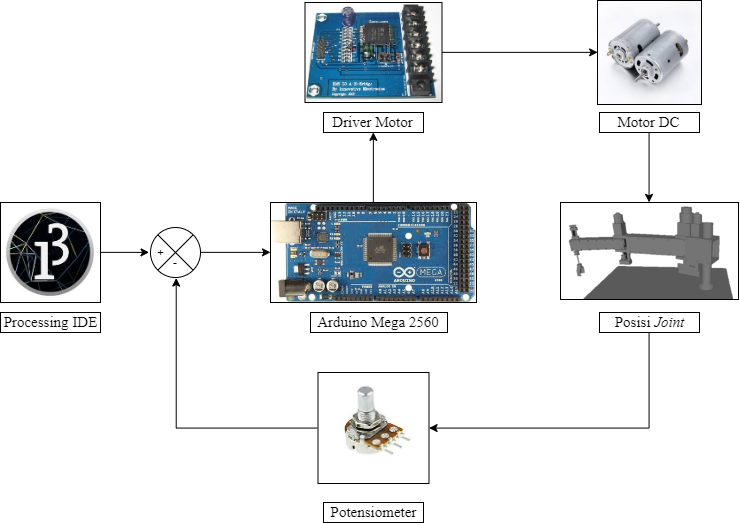
\includegraphics[width=12cm]{gambar/Rangkaian_Diagram.png}
	\caption{Diagram Blok Sistem}
\end{figure}
Pada blok diagram yang disajikan pada Gambar 3.1 sistem terdiri dari bagian – bagian yang meliputi bagian masukan, bagian kendali, bagian keluaran, dan bagian penampil. Pada bagian masukan menggunakan GUI yang dirancang pada Processing IDE yang digunakan sebagai \textit{forward kinematic} serta \textit{inverse kinematic} dimana robot akan bergerak menyesuaikan dengan posisi atau sudut yang diinputkan melauli Processing IDE. 
Pada bagian kontrol menggunakan Arduino Mega 2560 sebagai mikrokontroler yang mengendalikan seluruh operasi dari robot. \textit{Power supply} Arduino sebesar 5 volt DC didapatkan dari regulator tegangan yang menurunkan tegangan dari 12 volt DC ke 5 volt DC. 

Pada bagian keluaran, pin pulse with modulation (PWM) pada Arduino Mega 2560 dihubungkan dengan driver motor yang digunakan untuk mengontrol arah pergerakan dari motor DC serta kecepatan pergerakan dari motor DC. Pergerakan arah putaran motor DC bergantung pada \textit{feedback} posisi setiap sendi yang diberikan oleh potensiometer. Tiga buah pin digital ardunio dihubungkan rangkaian \textit{switch} yang menggunakan IC TIP31 yang berfungsi sebagai kontrol dari \textit{End-Effector} dari robot SCARA.

Pada bagian penampil merupakan bentuk dari rancangan GUI yang dirancang dalam Processing IDE melalui sebuah bentuk pemrograman. Dalam tampilan GUI nya, terdapat beberapa \textit{tools} yang dapat untuk mengatur pergerakan robot SCARA. Pada GUI juga dapat menampilkan nilai dari sudut, dan posisi pada kondisi langsung dari pergerakan robot SCARA.
\section{ Perancangan Perangkat Keras }
Perancangan perangkat keras pada \textit{arm manipulator robot} SCARA terdiri dari dua bagian yaitu bagian mekanik dan elektronis. Bagian  mekanik merupakan bagian \textit{hardware} yang meliputi desain, bahan dan bentuk dari arm manipulator robot SCARA dan bagian elektronis merupakan bagian \textit{hardware} yang meliputi sistem – sistem yang berkaitan dengan rangkaian pada I SCARA seperti rangkain pada desain \textit{board} serta komponen – komponen elektronis.
\subsection{ Sistem Mekanik }
Sistem mekanika dari robot lengan bergantung dari konfigurasi robot lengan. Konfigurasi robot lengan terbagi menjadi enam, yaitu konfigurasi \textit{Articulated}, konfigurasi SCARA, konfigurasi \textit{Spherical}, konfigurasi \textit{Cylindrical}, dan konfigurasi \textit{Cartesian}. Pada tugas ini, konfigurasi robot lengan yang digunakan adalah konfigurasi SCARA, dengan dua joint revolute dan satu \textit{end-effector}. Sistem mekanik dari lengan robot tiga DOF sangat berpengaruh dan mendominasi sistem karena bentuk dan pergerakan dari mekanik akan mempengaruhi elektronis, serta program. Sistem mekanik yang baik sangat mendukung dari pergerakan robot, oleh karena itu perancangan mekanik haruslah proporsional dari panjang setiap lengan, lebar serta tinggi robot. Pada Gambar 3.2 disajikan \textit{free body} dari robot SCARA dan Gambar 3.3 merupakan bentuk fisik dari robot SCARA yang digunakan pada penelitian kali ini.
\begin{figure}[H]
	\centering
	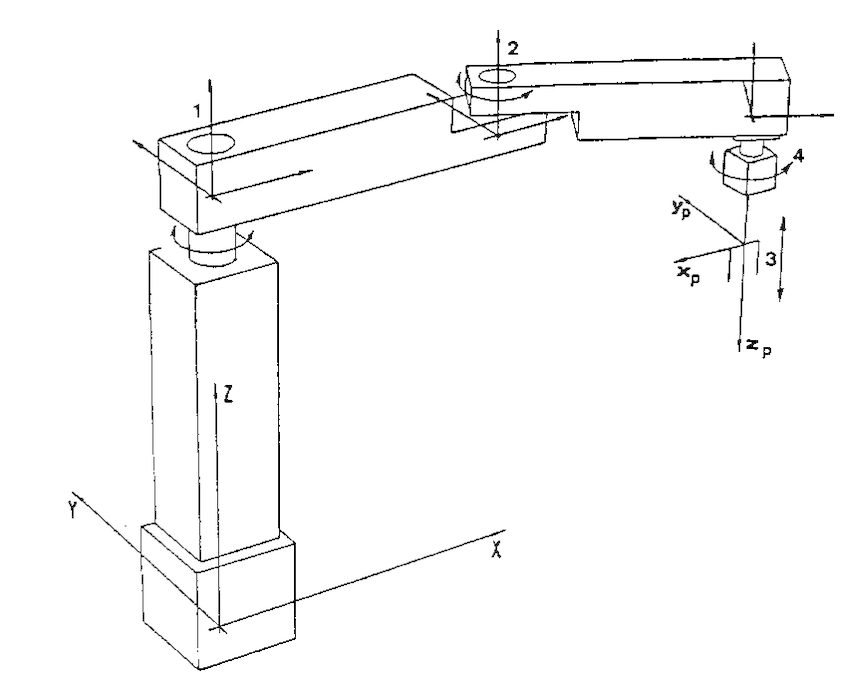
\includegraphics[width=7cm]{gambar/scaraa.png}
	\caption{\textit{Free Body} Robot SCARA}
\end{figure}
\begin{figure}[H]
	\centering
	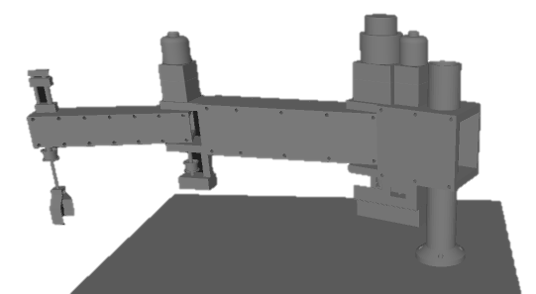
\includegraphics[width=7cm]{gambar/3dscara.png}
	\caption{Bentuk Fisik Robot SCARA}
\end{figure}
Robot SCARA merupakan robot yang meiliki tiga buah derajar kebebasan (DOF) yang terletak pada \textit{shoulder}, \textit{elbow}, dan pada \textit{end-effector}. Pada \textit{shoulder} dan \textit{elbow} menggunakan sebuah motor DC dan pada \textit{end-effector} menggunakan bantuan angin yang dikontrol penggunakan \textit{valve pneumatic.} Pergerakan pada masing-masing \textit{joint} memiliki jangkauan maksimum yang berbeda-beda. Jangkauan juga dipengaruhi oleh panjangnya lengan yang dimiliki oleh robot SCARA tersebut. Tabel 3.1 merupakan spesifikasi dari robot SCARA yang digunakan.


\begin{table}[H]
	\centering
	\caption{Spesifikasi Robot SCARA}
	
		\begin{tabular}{|l|l|}
			\hline
			Main arm length      & 360 mm		\\ \hline
			Fore arm length      & 290 mm  				\\ \hline
			Shoulder movement    & 180 °  		\\ \hline
			Elbow movement       & 200 °   		\\ \hline
			Wrist rotation       & 360 ° 		\\ \hline
			Up \& down movement  & 150 mm   				\\ \hline
			Maximum tip velocity & 3.0 kg  				\\ \hline
		\end{tabular} 
	\end{table}
Desain pada\textit{ arm manipulator robot} SCARA berbahan besi dengan tebal 2mm dengan tiga derajat kebebasan yang meliputi bagian \textit{shoulder}, \textit{elbow}, serta \textit{end-effector}. Pada desainnya robot SCARA terbagi menjadi dua bagian. Bagian utama adalah box panel yang berisi sistem elektronis utama dan pada bagian yang lain merupakan lengan dari robot SCARA sendiri. Terdapat juga tiga buah selang yang berfungsi untuk mentransformasikan angin untuk pergerakan dari \textit{end-effector} yang berasal dari sebuah kompresor.  Dalam komunikasinya dengan komputer personal, robot SCARA dihubungkan dengan konektor USB. Gambar 3.4 merupakan bentuk fisik dari box panel pada Robot SCARA.
\begin{figure}[H]
	\centering
	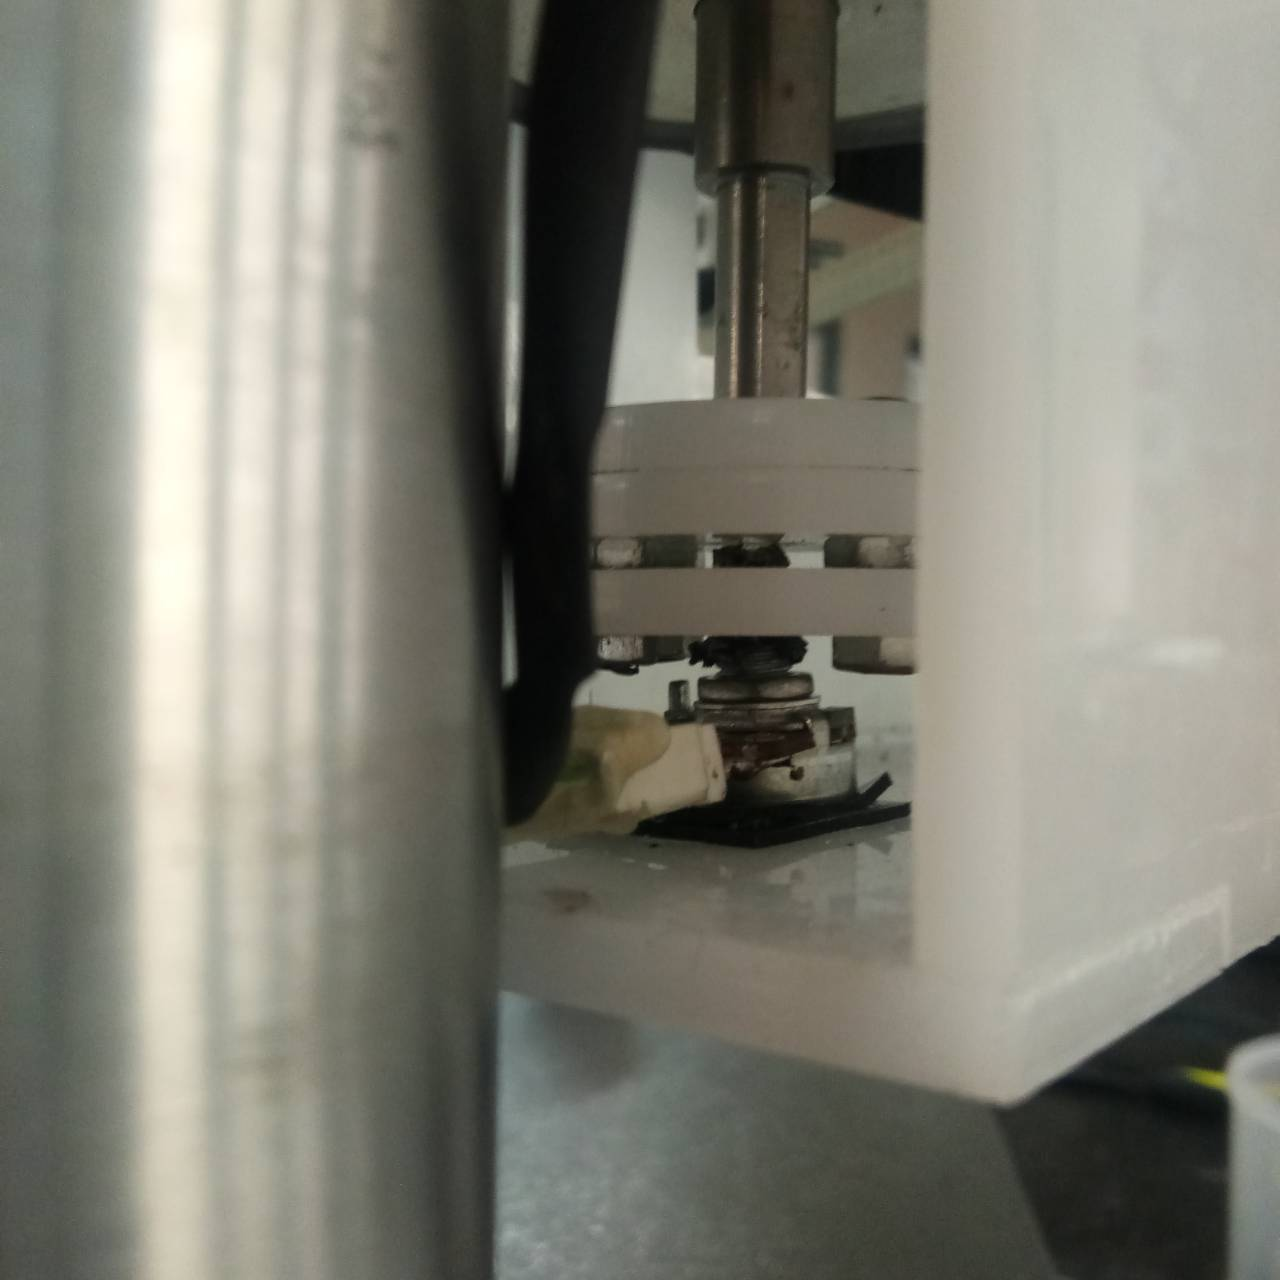
\includegraphics[width=5cm]{gambar/potsementara.jpg}
	\caption{Box Panel Robot SCARA}
\end{figure}

Pada \textit{arm manipulator robot} SCARA menggunakan penggerak berupa motor DC 12 Volt dengan diberikan \textit{gearbox} sehingga mampu mengangkat beban berat karena torsi pada motor bertambah besar. Motor DC dikontrol dari driver motor EMS 30A H-Bridge melalui mikrokontroler Arduino Mega 2560. Tabel 3.2 merupakan spesifikasi dari motor DC yang digunakan pada robot SCARA. 

	\begin{table}[H]
	\centering
	\caption{Spesifikasi Motor DC pada Robot SCARA}
	\resizebox{15cm}{!}{%
		\begin{tabular}{|l|l|}
			\hline
			Moments of inertia of the main arm ($J_{1}$)    							& $0.0980kgm^{2}$ 				\\ \hline
			Moments of inertia of the fore arm ($J_{2}$)    							& $0.0115 kgm^{2}$ 				\\ \hline
			Masses of the main arm	($m_{1}$)											& $1.90kg$   					\\ \hline
			Masses of the fore arm  ($m_{2}$)     										& $0.93kg$   					\\ \hline
			Motor and equivalent inertias ($J_{m}$)      								& $3.3*10^{-6}kgm^{2}$ 			\\ \hline
			Back emf constants for main arm and fore arm motor ($K_{e1}=K_{e2}$)  		& $0.047Nm/A$   				\\ \hline
			Armature resistance for main arm and fore arm motor($R_{a1}=R_{a2}$)		& $3.5\Omega$  					\\ \hline
			Armatures inductances for main and fore arm motor  ($L_{a1}=L_{a2}$) 		& $1.3mH$ 						\\ \hline
		\end{tabular}%
	}
\end{table}
%%
Pada bagian \textit{gearbox} pada masing-masing motor DC terdapat \textit{potensiometer} sebagai sensor posisi. \textit{Potensiometer} ditempatkan pada bawah motor DC yang terhubung langsung. Setiap pergerakan dari motor DC, \textit{potensiometer} akan secara otomatis juga ikut bergerak dan kemudian mengirimkan nilai data analog ke Arduino Mega. Nilai ini dalam Arduino Mega dilakukan sebuah perhitungan untuk menghasilkan sebuah posisi berupa besar sudut dari setiap motor DC saat dioperasikan. Gambar 3.5 merupakan bentuk fisik dari motor DC serta pemasangan \textit{potensiometer}.
\begin{figure}[H]
	\centering
	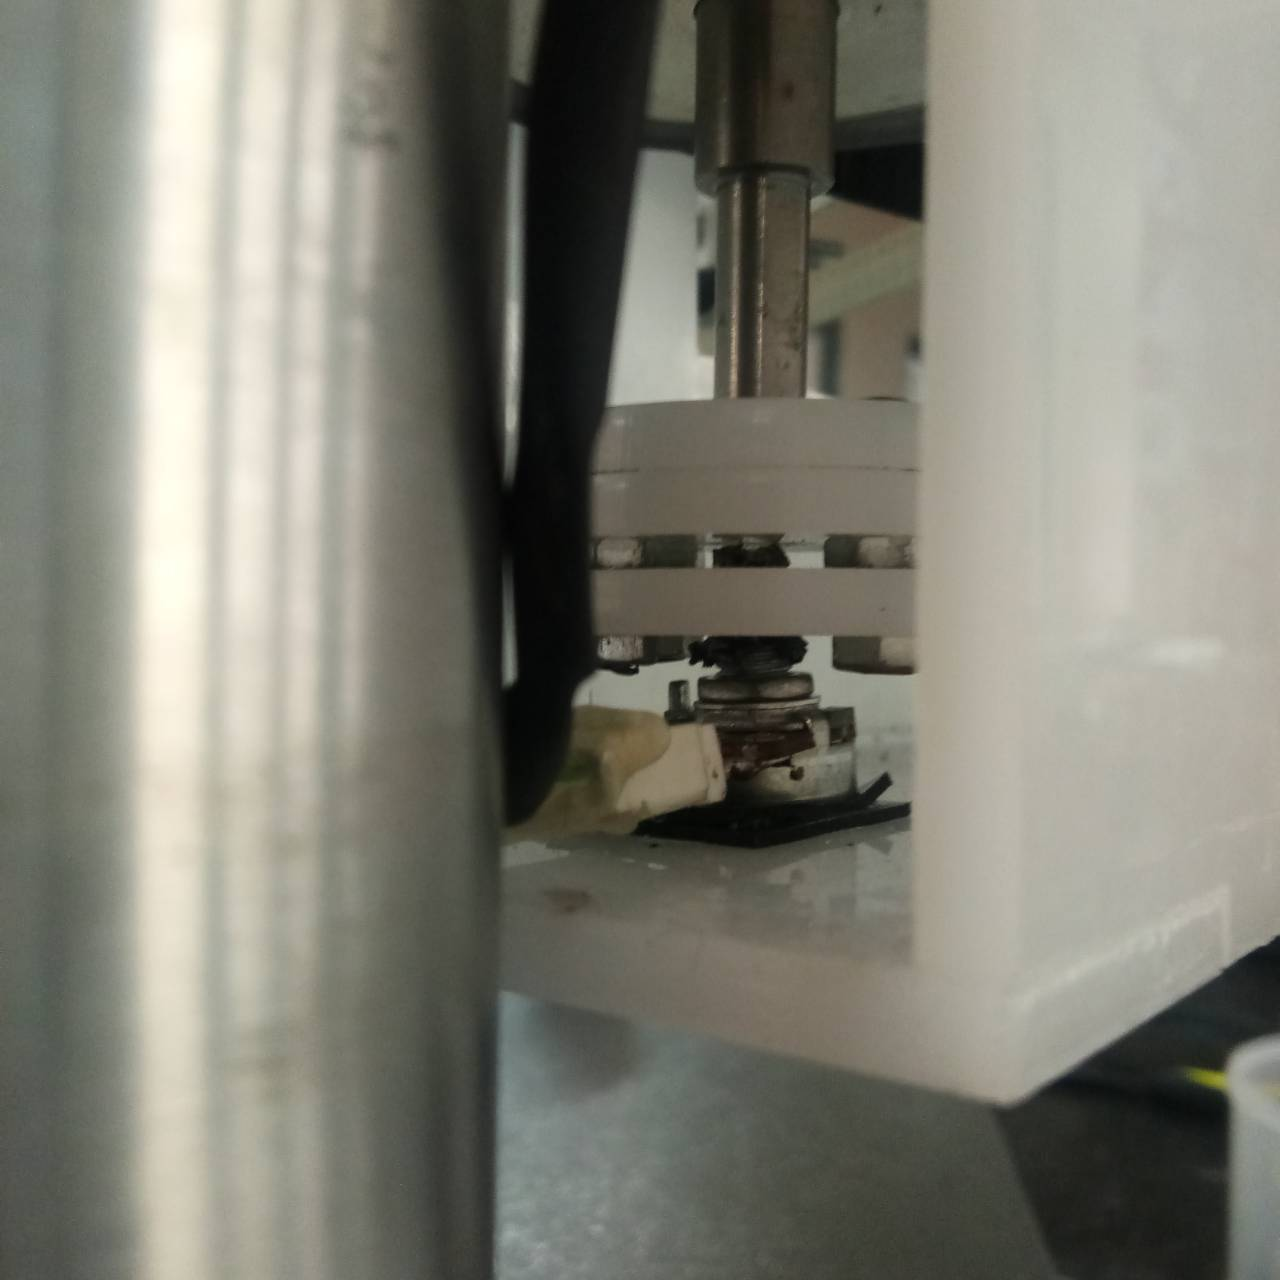
\includegraphics[width=5cm]{gambar/potsementara.jpg}
	\caption{Motor DC dengan Potensiometer}
\end{figure}

Pada bagian \textit{end-effetor} menggunakan pergerakan translasi. Pergerakan translasi merupakan pergerakan garis lurus dengan sebuah sumbu. Pada robot SCARA pergerakan ini ada pada bagian \textit{end-effector} yang bergerak secara vertikal atau naik turun. Dengan pergerakan ini, posisi \textit{end-effector} mengalami perubahan pada posisi tingginya. Pergerakan translasi juga terdapat pada bagian \textit{end-effector} yang menyebabkan sebuah\textit{ end-effector} dapat membuka dan menutup karena sebuah sistem mekanik yang telah ada. Selain dari pergerakan translasi, pergerakan pada end-effector juga terdapat rotasi. Pergerakan ini dilakukan oleh satu buah motor DC yang ditempatkan pada bagian base dengan dihubungkan melalui sebuauh belt. Pengoperasian pada motor DC ini juga dilakukan oleh driver motor EMS 30A H-Bridge. Gambar 3.6 merupakan bentuk fisik dari \textit{end-effector}. 
\begin{figure}[H]
	\centering
	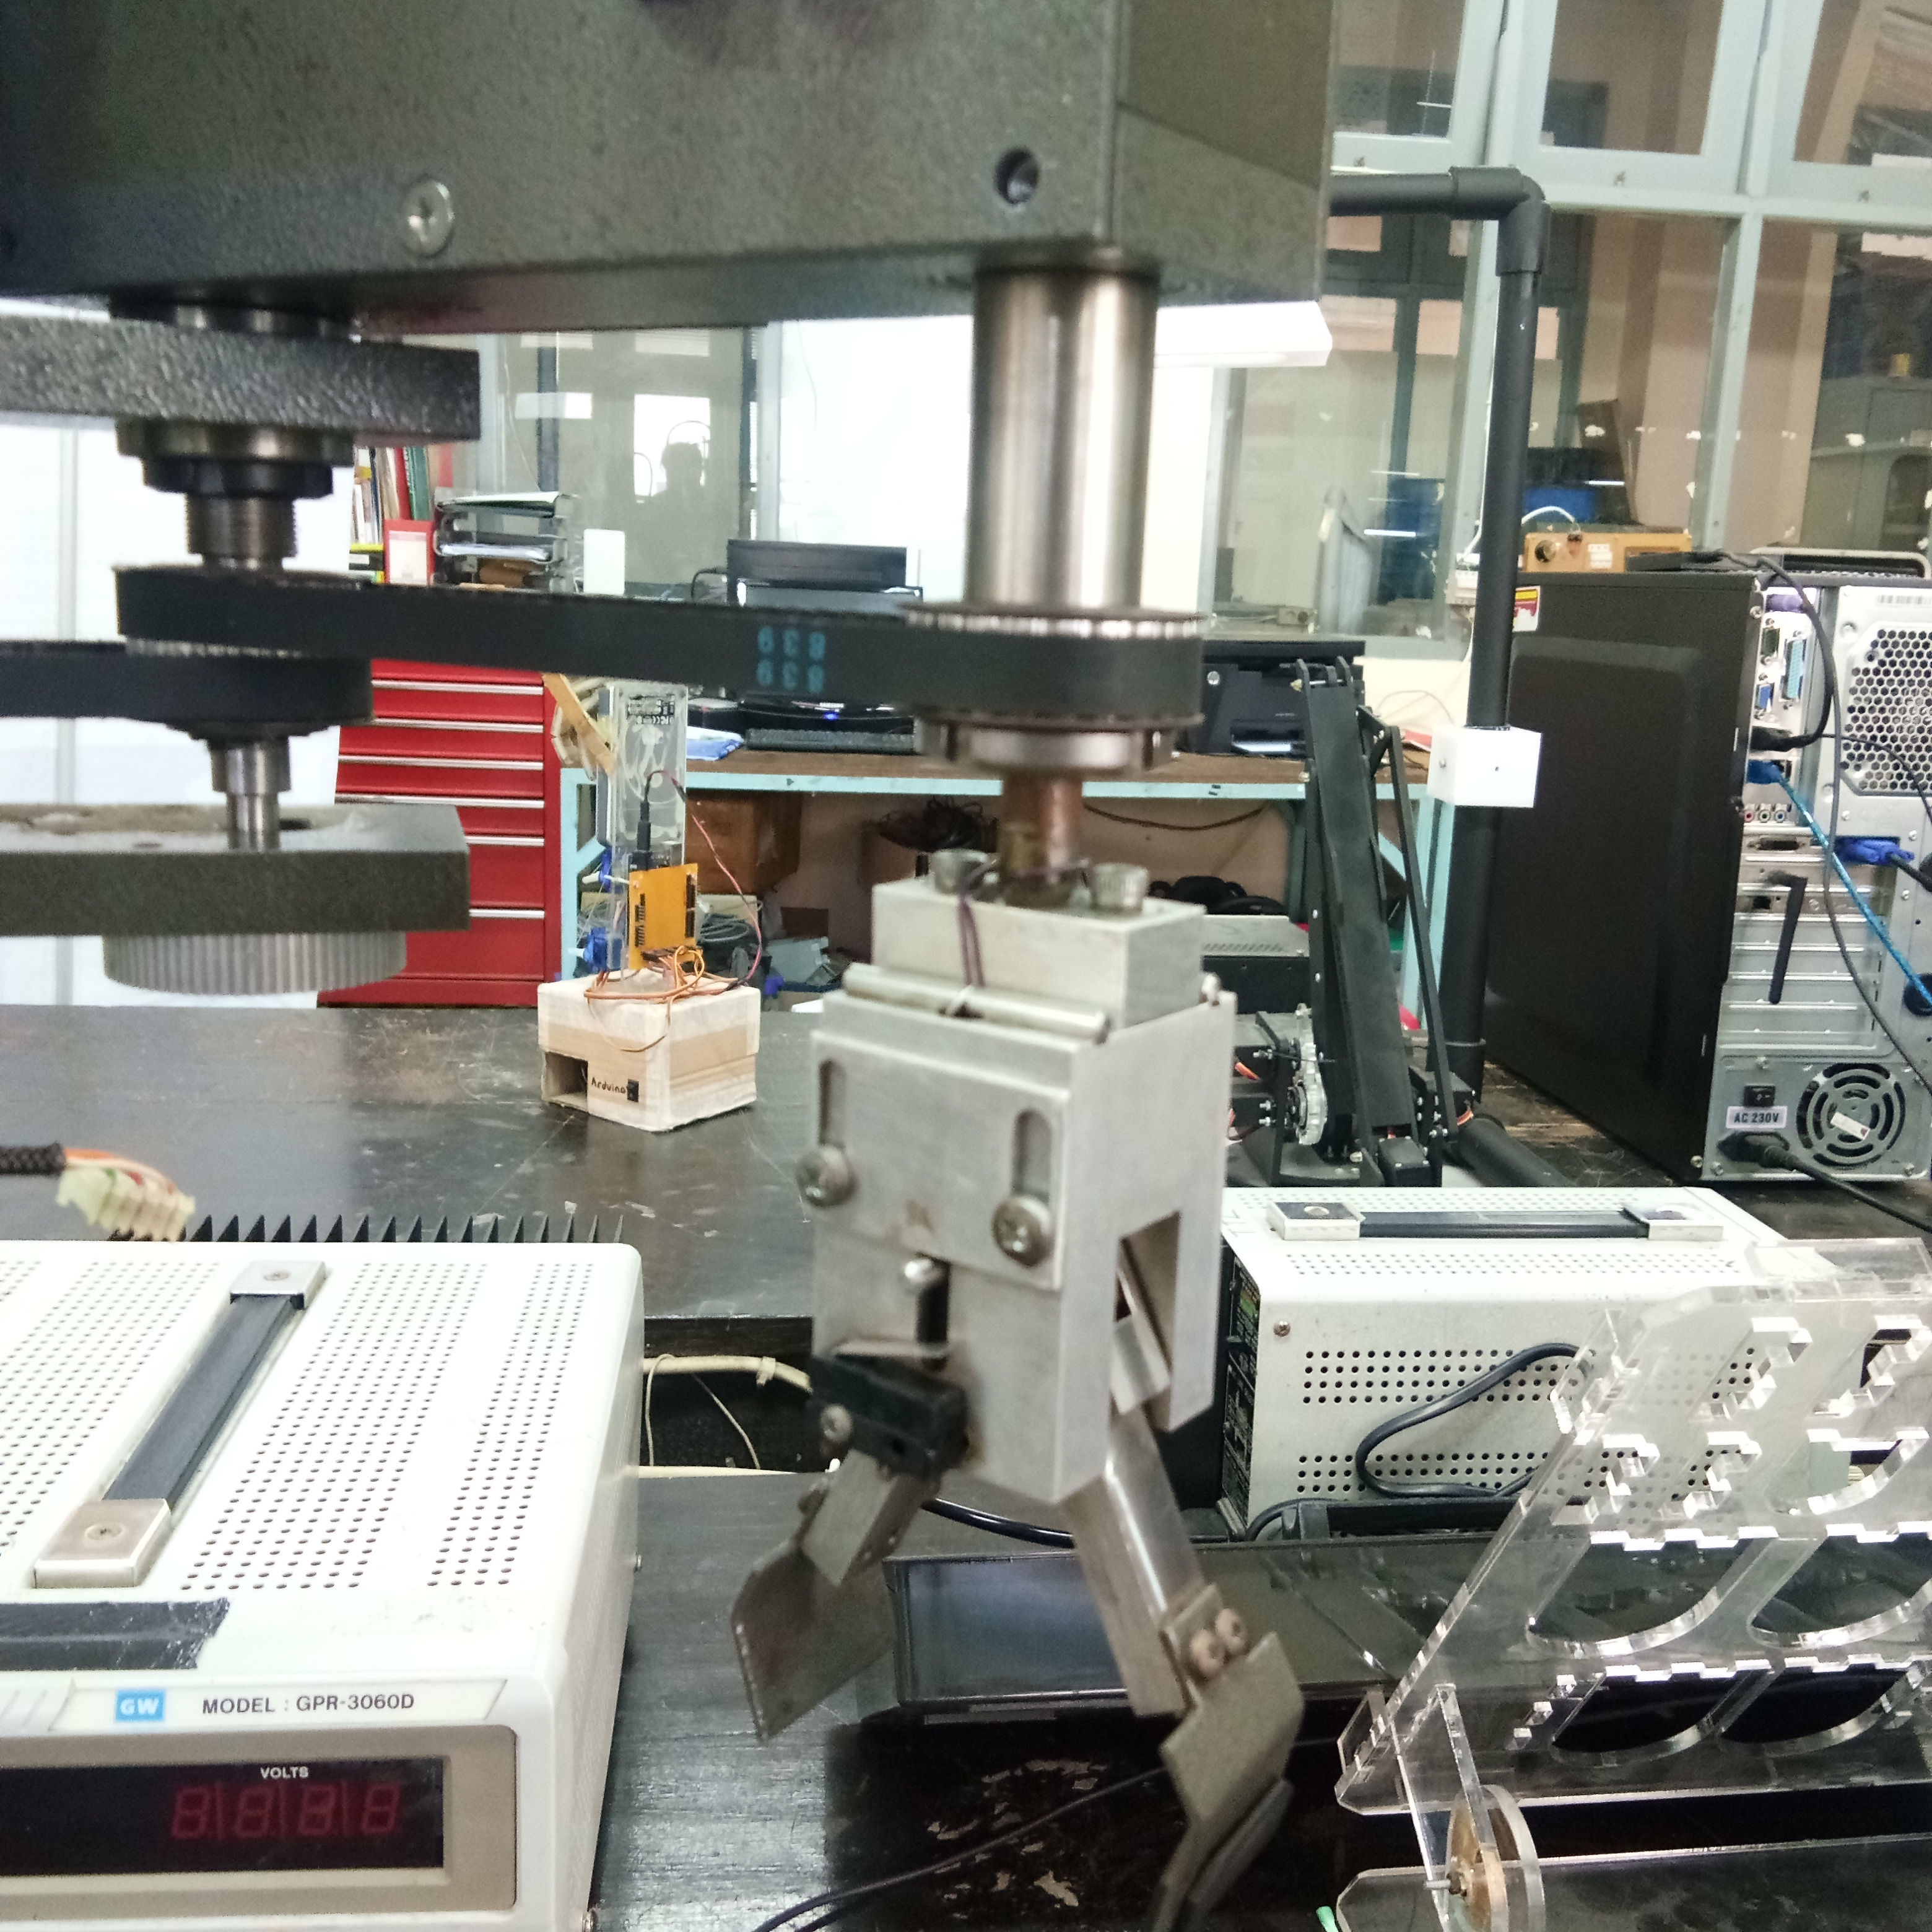
\includegraphics[width=5cm]{gambar/capitsementara.jpg}
	\caption{End-Effector Robot SCARA}
\end{figure}
Semua pergerakan pada \textit{end-effector} ditenagai oleh sebuah tekanan udara yang bersumber dari sebuah kompresor. Tekanan udara diaplikasikan pada sebuah \textit{pneumatic} dengan sistem kerja translasi yang dapat menyebabkan sebuah objek dapat bergerak pada sebuah garis lurus. Gambar 3.7 merupakan bentuk fisik dari pneumatic yang digunakan pada robot SCARA. 
\begin{figure}[H]
	\centering
	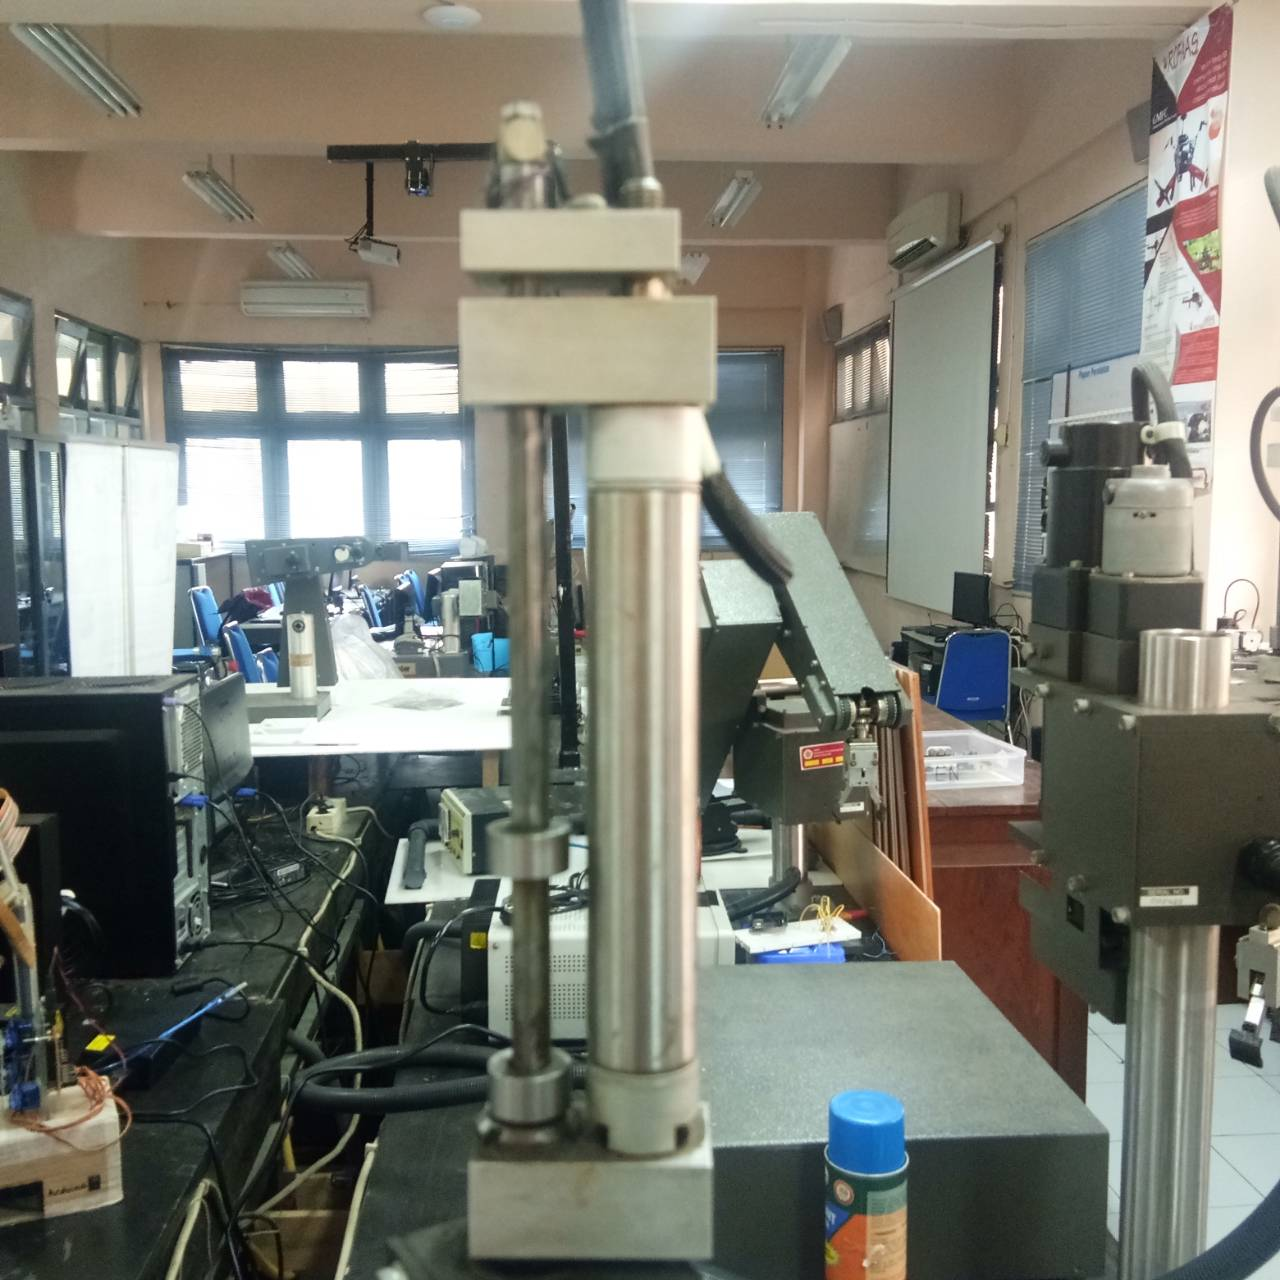
\includegraphics[width=5cm]{gambar/penuamticsementara.jpg}
	\caption{Bentuk Fisik Pneumatic}
\end{figure}
Kompresor yang digunakan untuk menghasilkan sebuah tekanan udara merupakan sebuah kompresor listrik dengan kapasitas 8 bar. Kompresor ini dioperasikan menggunakan sumber tegangan AC. Ketika kapasitas udara sudah terpenuhi, kompresor ini dapat digunakan tanpa menggunakan sumber tegangan tetapi hanya sebatas kapasitas udara yang disimpan. Gambar 3.8 merupakan bentuk kompresor yang digunakan.
\begin{figure}[H]
	\centering
	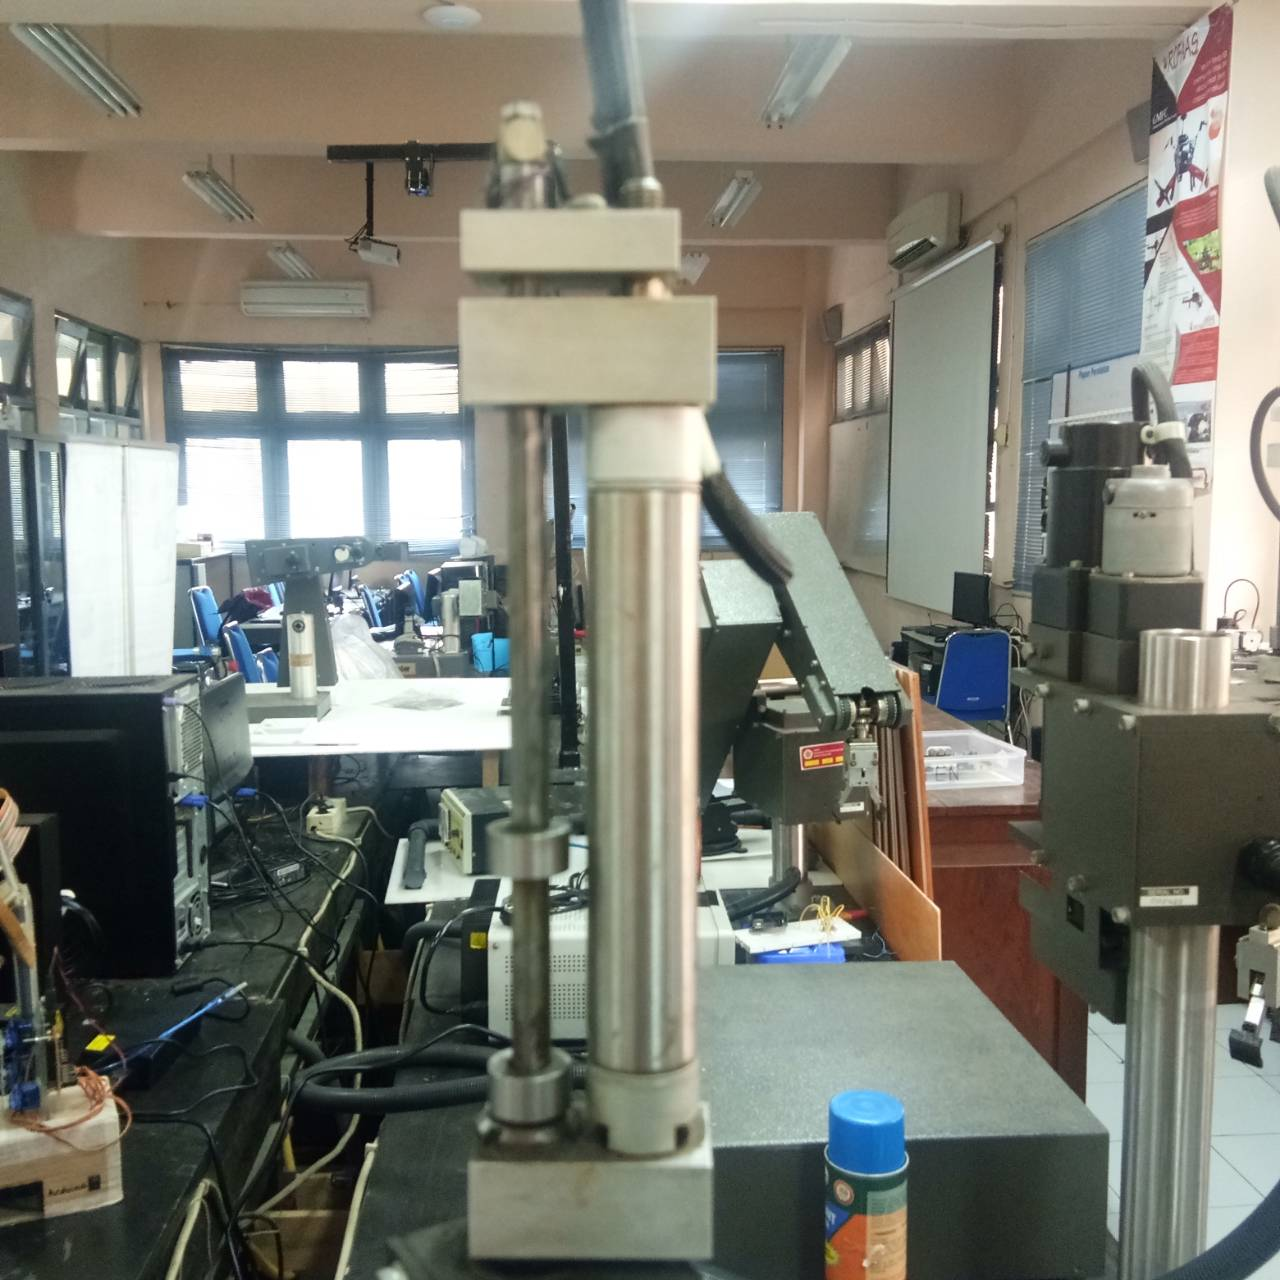
\includegraphics[width=5cm]{gambar/penuamticsementara.jpg}
	\caption{Bentuk Fisik Kompresor}
\end{figure}

Rancangan robot secara keseluruhan ditampilan pada Gambar 3.9 yang merupakan rancangan tampak samping, Gambar 3.10 merupakan rancangan tampak atas dan Gambar 3.11 merupakan rancangan dimensi robot. 
\begin{figure}[H]
	\centering
	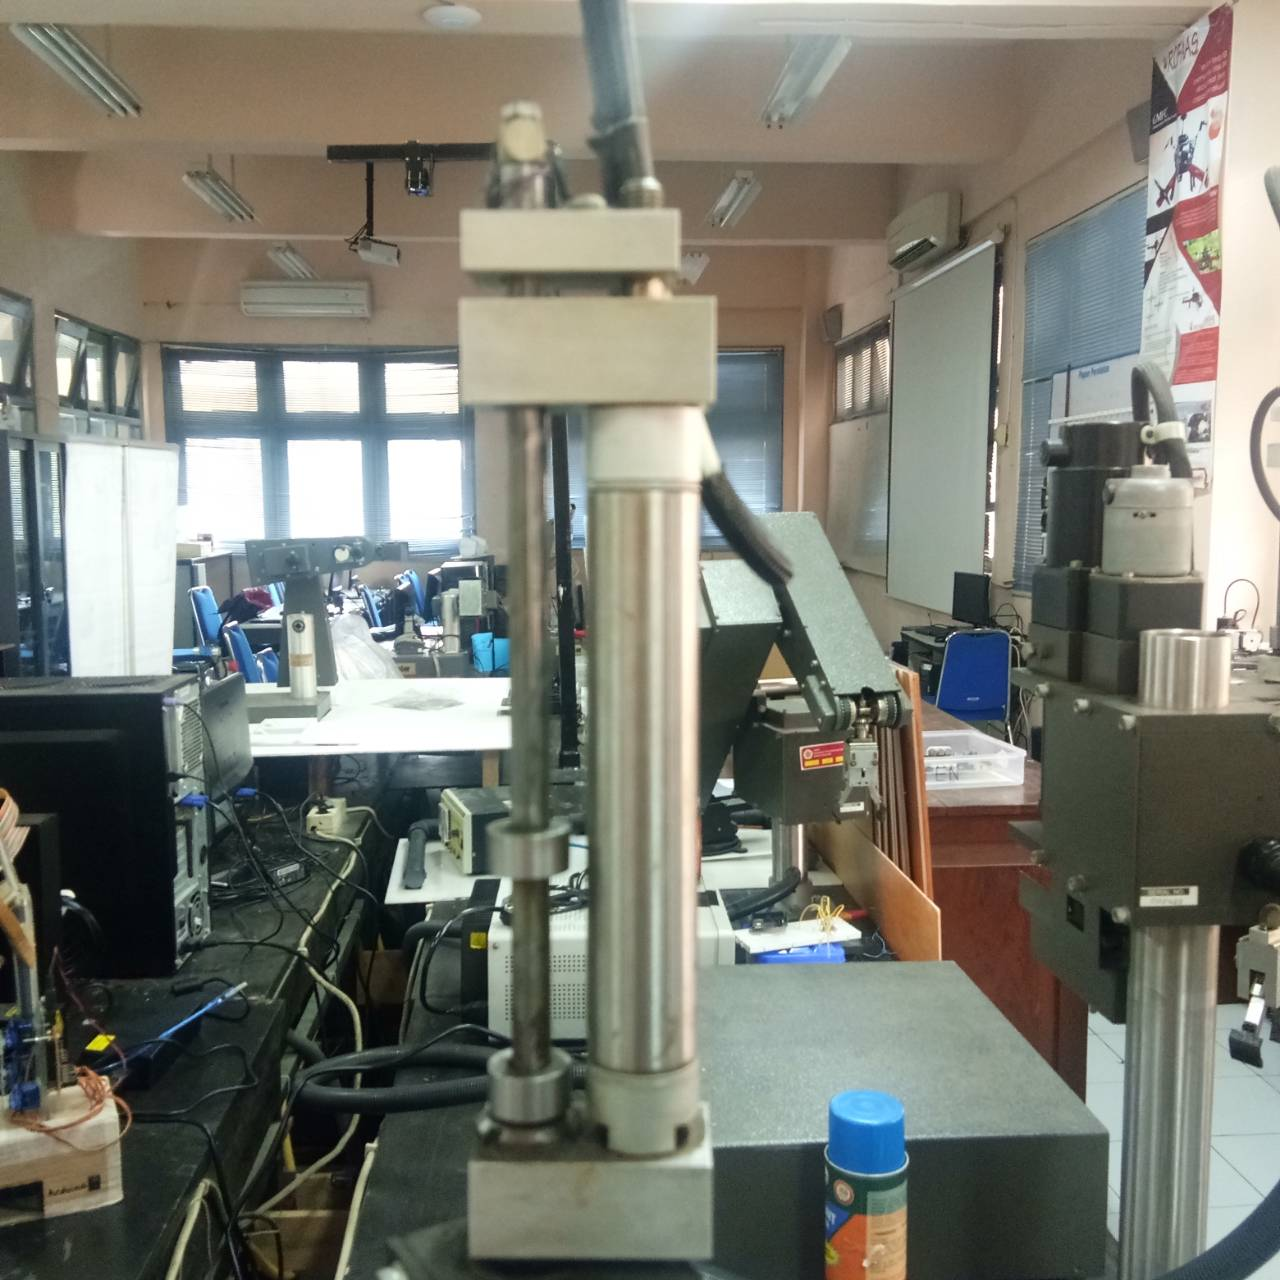
\includegraphics[width=5cm]{gambar/penuamticsementara.jpg}
	\caption{Rancangan Tampak Samping}
\end{figure}

\begin{figure}[H]
	\centering
	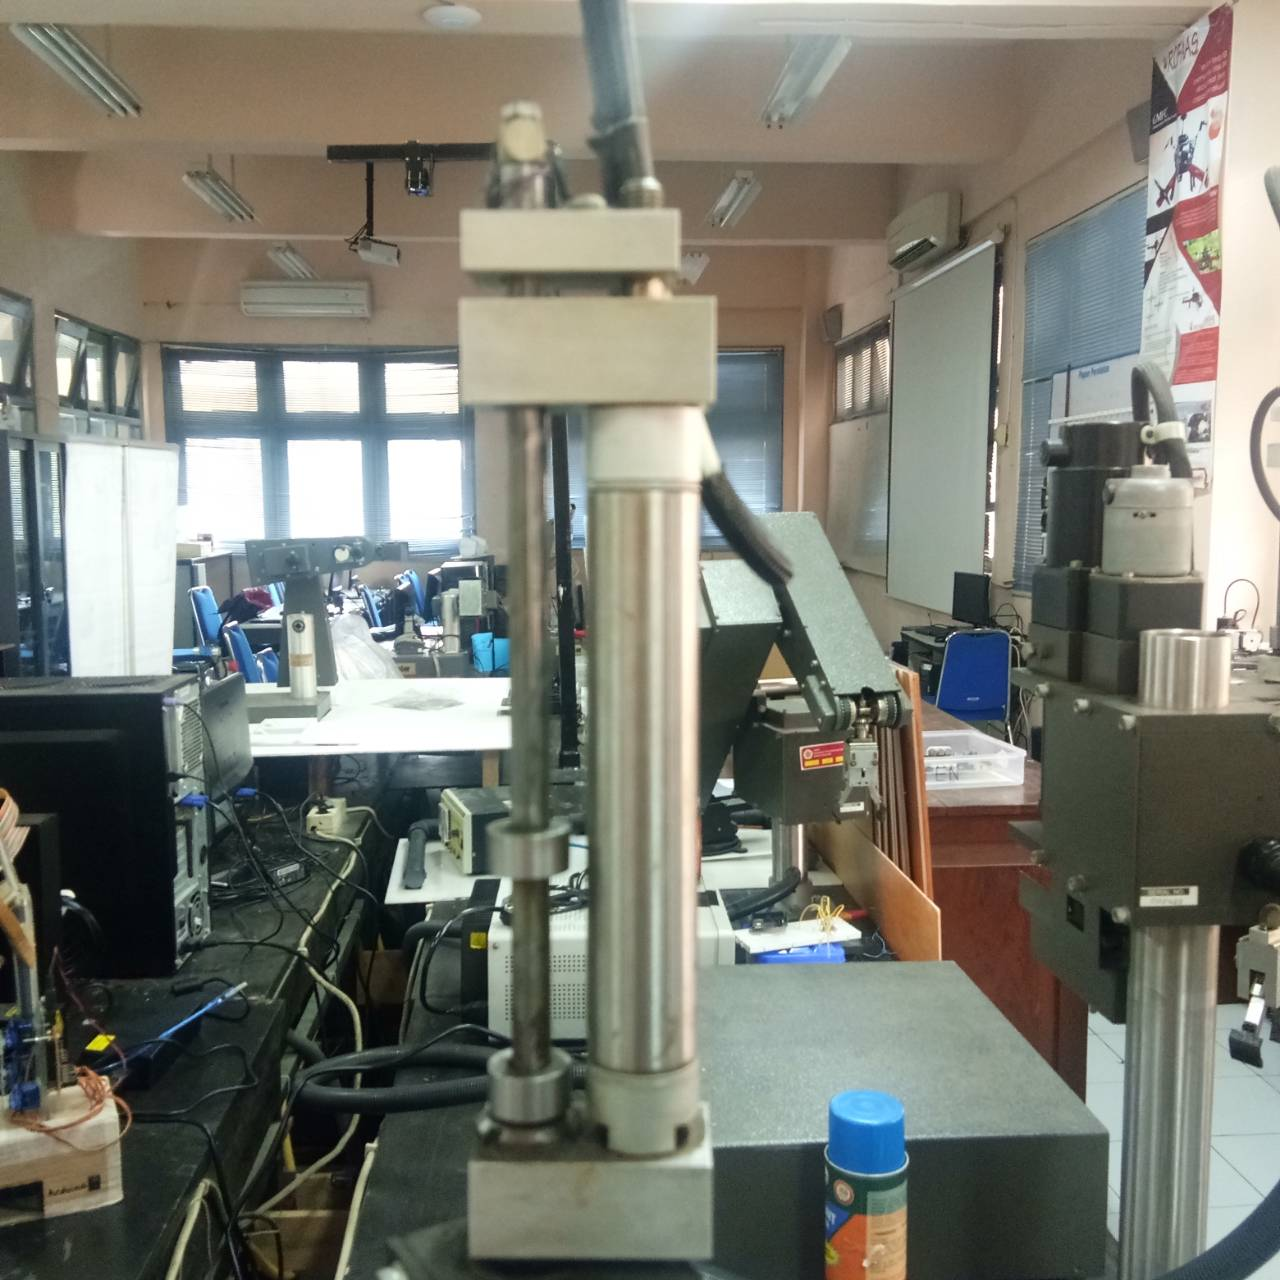
\includegraphics[width=5cm]{gambar/penuamticsementara.jpg}
	\caption{Rancangan Tampak Atas}
\end{figure}

\begin{figure}[H]
	\centering
	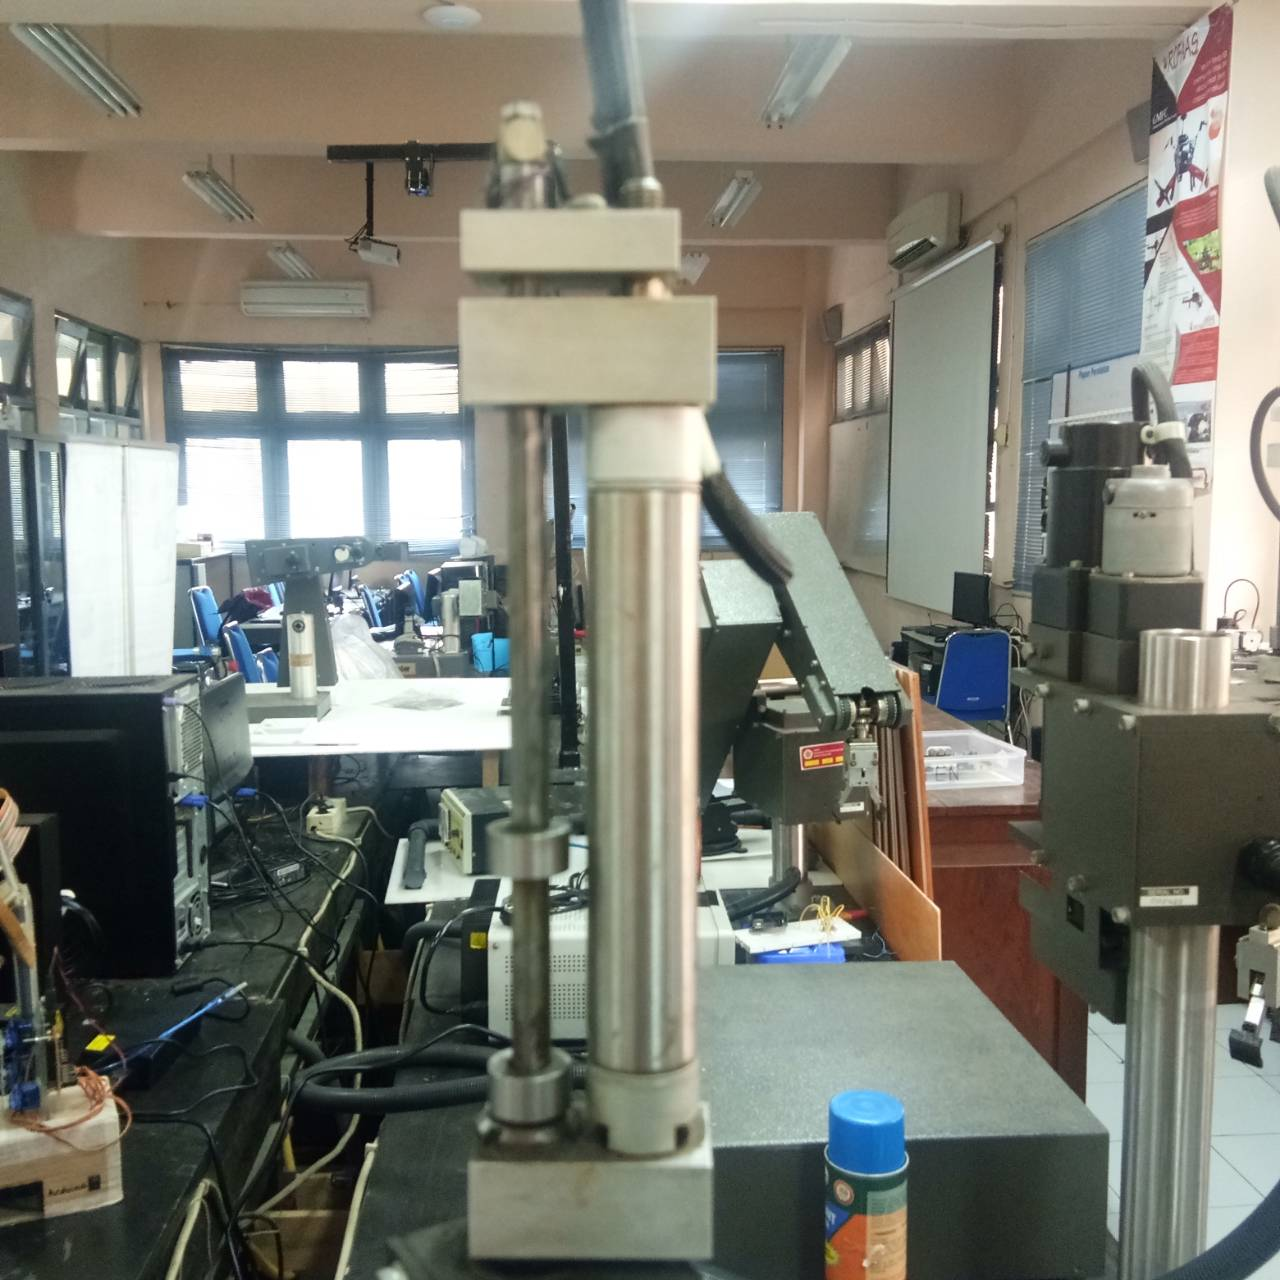
\includegraphics[width=5cm]{gambar/penuamticsementara.jpg}
	\caption{Dimensi Robot}
\end{figure}

\subsection{Rangkaian Elektronika}
\subsubsection{Rangkaian Motor DC}
Rancangan kendali pada \textit{arm manipulator robot} SCARA ini menggunakan tiga buah motor DC dengan masing – masing dilengkapi dengan \textit{gearbox} untuk memperkuat torsi yang dihasilkan oleh motor DC. Pada  \textit{gearbox} masing – masing motor  DC diberikan sensor \textit{potensiometer} sebagai \textit{feedback} untuk memberikan posisi motor DC pada keseluruhan sistem. Motor DC diletakkan pada \textit{base} untuk \textit{end-effector} satu buah, pada \textit{shoulder} satu buah, dan pada \textit{elbow} satu buah. Ketiga motor DC tersebut masing-masing menggunakan driver motor EMS 30A H-Bridge dalam sistem kerjanya. Pada masing – masing motor DC membutuhkan catu daya antara 12 Volt DC. Rangkaian driver motor mendapat sumber tegangan DC 12V untuk disalurkan ke pada motor nya dan 5V untuk kerja dari driver motor sendiri. 12V di dapat dari tegangan keluaran yang dihasilkan oleh regulator \textit{Buck} yang berseumber dari tegangan DC 24V. Ragkaian utama driver motor EMS 30A H-Bridge ditunjukkan pada Gambar 3.12 dan pada Gambar 3.13 merupakan rangkaian antara motor DC, driver motor, dan Arduino Mega.  
\begin{figure}[H]
	\centering
	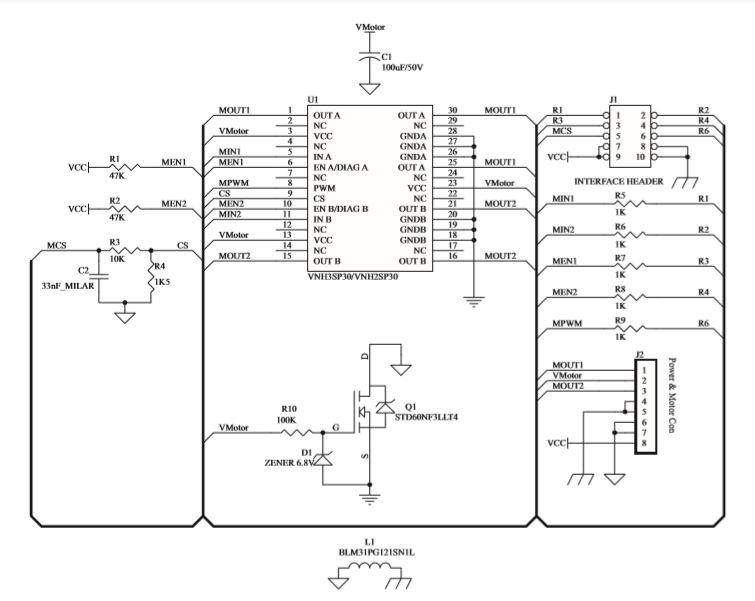
\includegraphics[width=10cm]{gambar/rangakaiandriver.jpg}
	\caption{Rangkaian Utama Driver Motor EMS 30A H-Bridge}
\end{figure}
\begin{figure}[H]
	\centering
	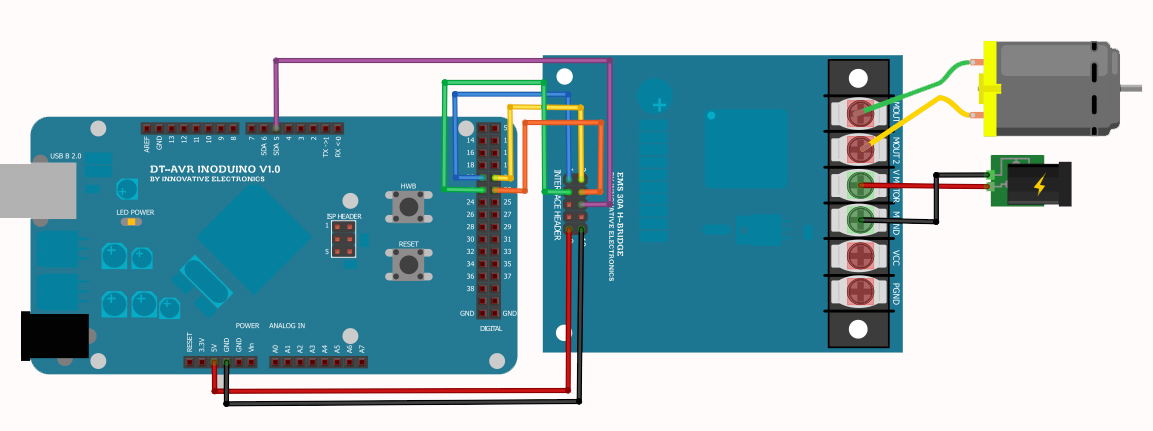
\includegraphics[width=10cm]{gambar/drivermotor.jpg}
	\caption{Rangkaian Arduino antara Driver Motor dan Motor DC}
\end{figure}
\subsubsection{Rangkaian \textit{Valve Relay Pneumatic}}
\textit{End-Effector} menggunakan tekanan udara dalam melakukan pergerakannya. Tekanan udara ini dikontrol menggunakan sebuah\textit{valve relay}. \textit{Valve relay} yang digunakan dapat mengkontrol tekanan udara hingga delapan bar. \textit{Valve relay} dapat bekerja pada tegangan DC 24 Volt. Tegangan 24 Volt pada \textit{valve relay} didapat dari keluaran dari rangkaian AC-DC yang dilakukan oleh dioda bridge dengan masukan awalnya adalah tegangan AC 24 Volt yang diberikan oleh sebuah trafo. Dengan besaran tegangan 24 Volt maka sebuah arduino tidak dapat mengkontrolnya. Oleh karena itu, diberi sebuah rangkaian pembantu yang prinsipinya bekerja seperti saklar. Rangkaian tersebut diotaki oleh IC TIP31A yang nantinya akan menerima sinyal data digital dari Arduino dan akan membuka jalur untuk tegangan 24Volt. Gambar 3.14 merupakan bentuk fisik dari \textit{valve relay} yang digunaakan dan Gambar 3.15 merupakan rangkaian dari valve relay dengan rangkaian TIP31A.
\begin{figure}[H]
	\centering
	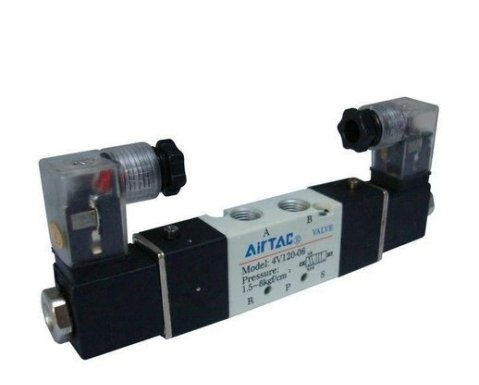
\includegraphics[width=7cm]{gambar/relay.jpg}
	\caption{Bentuk Fisik dari Valve Relay}
\end{figure}
\begin{figure}[H]
	\centering
	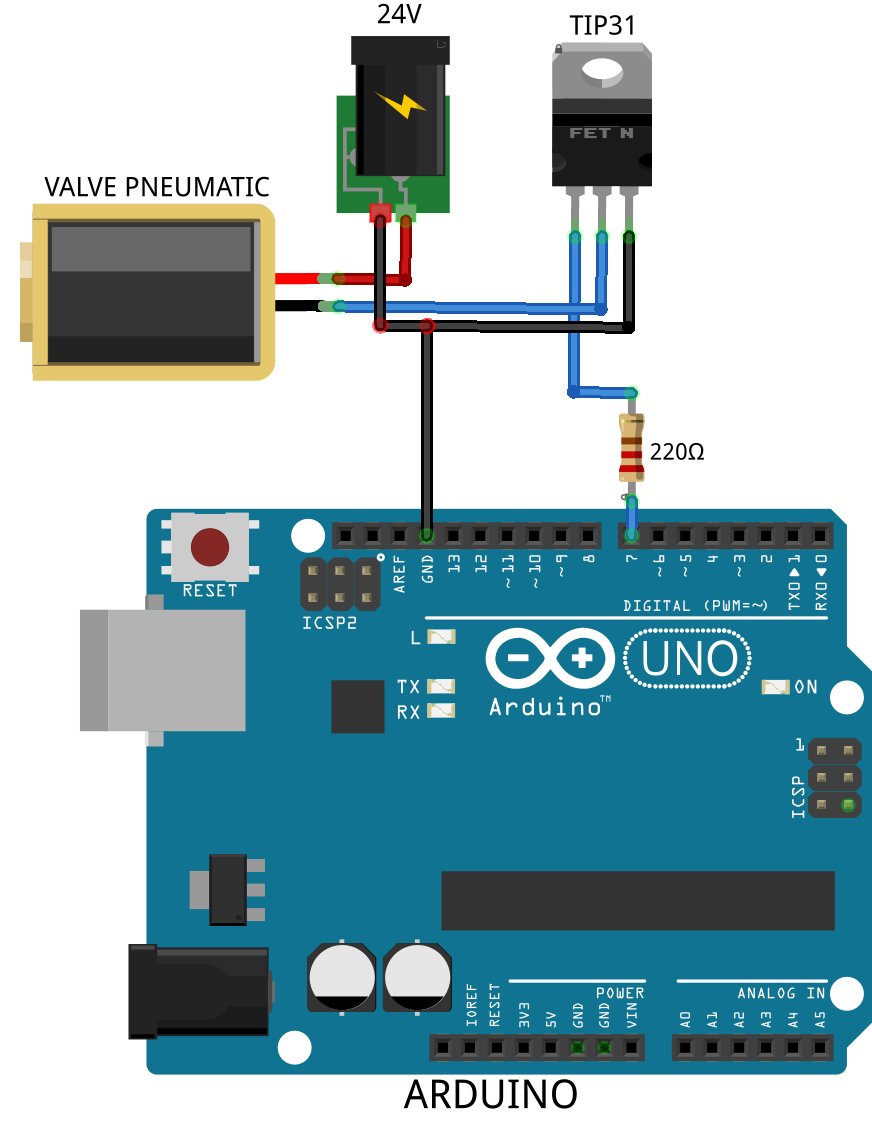
\includegraphics[width=7cm]{gambar/tip31.png}
	\caption{Rangkaian Valve Relay dengan Rangkaian TIP31}
\end{figure}
\subsubsection{Rangkaian Minimum Sistem Arduino}
Arduino  2560 digunakan sebagai mikrokontroler utama untuk mengendalikan seluruh sistem pada arm manipulator robot SCARA. Arduino  2560 memiliki banyak pin keluaran dan masukan digital dan analog yang dapat digunakan sebagai pengendali fungsi – fungsi dari setiap komponen. Pin pada Arduino  2560 dapat mencukupi kebutuhan masukan dan keluaran untuk sistem kerja robot. Pin analog yang pada Arduino  digunakan untuk menerima feedback masukkan dari potensio yang ada pada setiap motor robot. Beberapa pin digital pada Arduino  2560 juga  memiliki fungsi lain yaitu sebagai pin pulse with modulation (PWM) yang dapat digunakan sebagai keluaran analog sehingga dapat digunakan untuk mengatur nilai tegangan kaluaran dari Arduino  2560. Pin PWM yang cukup digunakan untuk kontrol kecepatan pada driver motor, selain itu pin PWM pada Arduino  2560 digunakan untuk memberikan kontrol direksi pada driver motor untuk memberikan masukan arah putar kanan ataupun putar kiri. Rangkaian minimum sistem arduino ditunjukkan pada Gambar 3.16 dan fungsi dari masing – masing pin Arduino  2560 dijelaskan pada tabel Tabel 3.2. 
\begin{figure}[H]
	\centering
	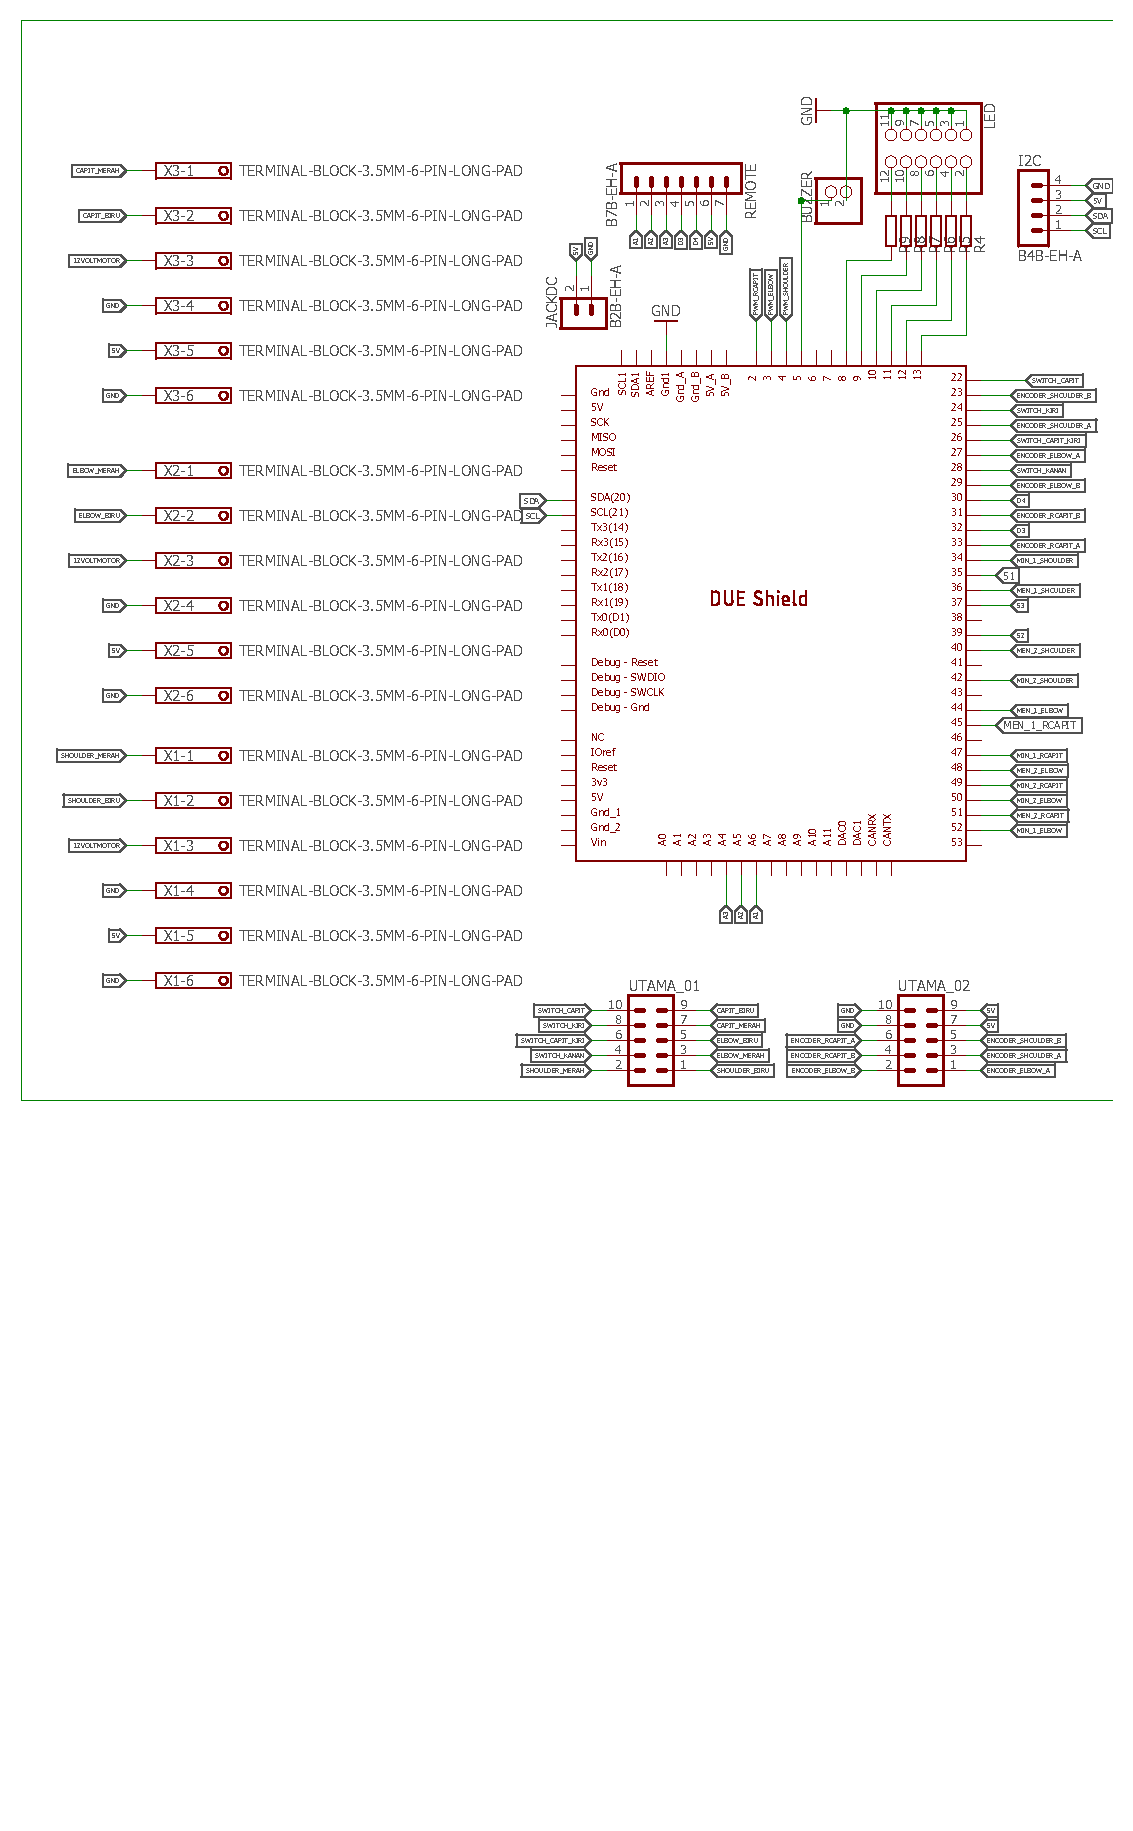
\includegraphics[width=15cm]{gambar/skematik.pdf}
	\caption{Rangkaian Minimum Sistem Arduino}
\end{figure}

\begin{table}[H]
		\centering
	\caption{Pin pada Arduino Mega 2560}
	\begin{tabular}{|c|c|l|}
		\hline
		\rowcolor[HTML]{9B9B9B} 
		No & \begin{tabular}[c]{@{}c@{}}Pin Arduino\\   Mega 2560\end{tabular} & \multicolumn{1}{c|}{\cellcolor[HTML]{9B9B9B}Fungsi} \\ \hline
		1  & A1                                                                & Feedback potensiometer shoulder                     \\ \hline
		2  & A2                                                                & Feedback potensiometer elbow                        \\ \hline
		3  & A3                                                                & Feedback potensiometer end-effector                 \\ \hline
		4  & D16, D18                                                          & Kontrol aktif driver motor shoulder                 \\ \hline
		4  & D20, D22                                                          & Kontrol driver motor shoulder                       \\ \hline
		5  & D24, D26                                                          & Kontrol aktif driver motor elbow                    \\ \hline
		6  & D28. D30                                                          & Kontrol driver motor elbow                          \\ \hline
		7  & D32, D34                                                          & Kontrol aktif driver motor end-effector             \\ \hline
		8  & D36, D38                                                          & Kontrol driver motor end-effector                   \\ \hline
		9  & D4                                                                & Kontrol PWM driver motor shoulder                   \\ \hline
		10 & D5                                                                & Kontrol PWM driver motor elbow                      \\ \hline
		11 & D6                                                                & Kontrol PWM driver motor end-effector               \\ \hline
		12 & D7                                                                & Kontrol valve relay naik                            \\ \hline
		13 & D8                                                                & Kontrol valve relay turun                           \\ \hline
		14 & D9                                                                & Kontrol valve relay buka-tutup                      \\ \hline
		15 & D15                                                               & Kontrol LED Shoulder aktif high                     \\ \hline
		16 & D17                                                               & Kontrol LED elbow aktif high                        \\ \hline
		17 & D19                                                               & Kontrol LED end-effector naik aktif high            \\ \hline
		18 & D21                                                               & Kontrol LED end-effector turun aktif high           \\ \hline
		19 & D23                                                               & Kontrol LED end-effector buka-tutup aktif high      \\ \hline
		20 & D25                                                               & Buzzer aktif high                                   \\ \hline
	\end{tabular}
\end{table}

\subsubsection{Rangkaian Catu Daya}
Rangkaian catu daya merupakan hal yang sangat penting agar semua kompononen pada robot dapat bekerja sesuai dengan fungsi yang telah dirancang. Pada \textit{arm manipulator robot} SCARA komponennya terdapat tiga buah besar tegangan \textit{supply} yang berbeda. Arduino Mega 2560 dan beberapa sensor membutuhkan tegangan 5 Volt, motor DC membutuhkan tegangan 12 Volt dan \textit{valve relay} membutuhkan 24 Volt. Catu daya diawali dengan tegangan AC 220 Volt dari listrik PLN. Tegangan tersebut kemudian diturunkan menggunakan sebuah trafo 3A menjadi 24 Volt AC. Komponen yang digunakan dalam rangakaian merupakan komponen yang membutuhkan tegangan DC, maka tegangan 24 Volt AC diubah menjadi 24 DC menggunakan rangkaian dioda \textit{bridge}. Tegangan 24 Volt DC diarahkan menuju dua buah regulator \textit{Buck} LM2596 yang masing-masing menghasilkan tegangan 12 Volt dan 5 Volt. Gambar 3.18 merupakan rangkaian catu daya secara keseluruhan.
\begin{figure}[H]
	\centering
	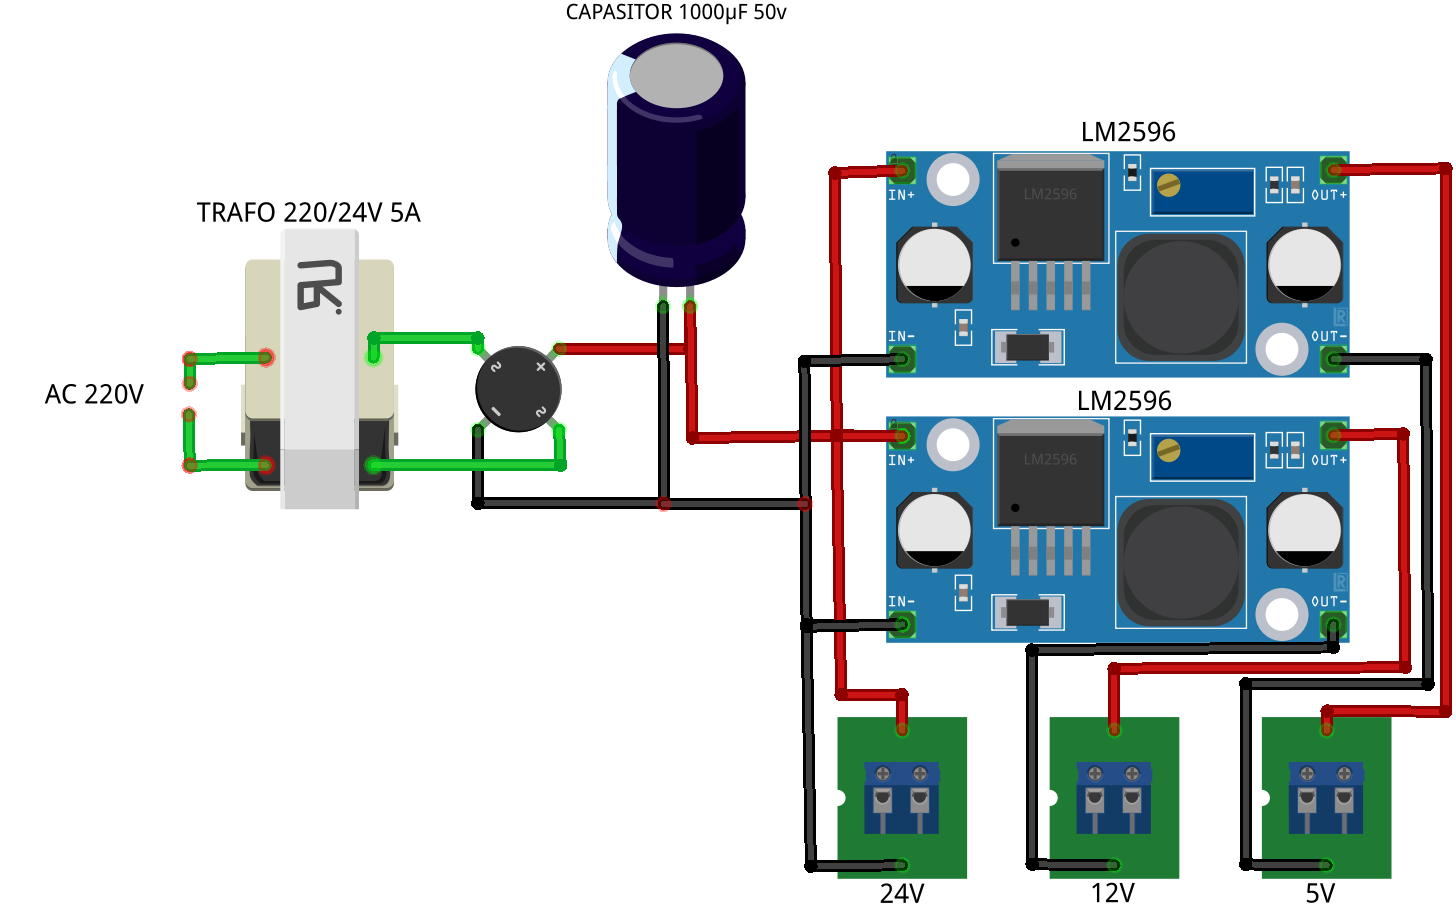
\includegraphics[width=8cm]{gambar/catudaya_bb.png}
	\caption{Rangkaian Catu Daya}
\end{figure}
\subsection{Perancangan Perangkat Lunak}
Perangkat lunak yang digunakan merupakan \textit{software} Processing IDE. Processing IDE diprogram agar mendapatkan sebuah GUI yang cocok sesuai dengan fungsi robot SCARA. Di dalam GUI terdapat dua bagian yang diantaranaya merupakan bagian kontrol, dan bagian \textit{display}. Pada bagian kontrol nantinya dalam GUI akan mengkontrol mulai dari pergerakan dan posisi dari robot SCARA. Sedangkan pada bagian penampil, GUI menampilkan nilai dari sudut, posisi, serta animasi terkait robot SCARA.
\subsubsection{ControlP5}
ControlP5 merupakan salah satu library yang berguna dalam membuat sebuah GUI. Dalam library yang disediakan terdapat banyak pilihan terkait kontrol sistem dengan berbagai jenis pilihan. Kontrol sistem yang disediakan tersedia dua pilihan yaitu untuk menkontrol dan untuk menampilkan sebuah data. Masing-masing kontrol sistem ini dapat digunakan dengan cara memanggilnya pada program yang ditulis.

Pada perancangan kineatika roboto scara ini, menggunakan empat buah kontrol sistem. Empat kontrol sistem yang digunakan merupakan jenis kontrol sistem yang berguna untuk memberikan sebuah data yang dikirimkan pada Arduino Mega 2560. Kontrol sistem tersebut diantaranya:
\begin{enumerate}
	\item \textit{Slider Control} \\
	\textit{Slider Control} berupa tampilan kontrol GUI yang menggunakan sistem geser dalam memberikan data. Data memiliki batasan atas dan batas bawah yang dimasukkan dalam program. Keuntungan menggunakan kontrol sistem jenis ini karena saat ingin untuk mengubah data yang diberikan menjadi lebih mudah.


	\item \textit{Textfield Control} \\
\textit{Textfield control} berupa tampila kontrol GUI yang menggunakan masukan nilai data sesuai apa yang dituliskan atau diketikkan secara langsung. Kelebihan menggunakan kontrol sistem jenis ini karena dapat memasukkan nilai data lebih spesifik secara langsung sesuai keiinginan.
	
	\item \textit{Textfield Control} \\
\textit{Bang control}
Berbeda dengan kontrol sistem sebelumnya,\textit{ bang control }berupa kotak yang bekerja pada saat mulai ditekan. Saat bang mulai ditekan data akan dikirimkan sesuai dengan nilai yang sudah dimasukan kedalam program. 
	

	\item \textit{Textfield Control} \\
\textit{Toggle control}
Toggle control memiliki sistem kontrol seperti saklar on-off. Pada saat ditekan maka toggle control menyimpan data berupa kondisi pertama dan berubah saat ditekan kembali. 

\end{enumerate}
\subsubsection{Shape}
Shape pada GUI berfungsi sebagai penampil secara tiga dimensi dari robot SCARA. Robot SCARA dapat ditampilkan dalam berbagai ukuran, letak dan juga dapat bergerak sesuai dengan data yang diberikan. Pergerakan dari robor SCARA merupakan implementasi dari wujud aslinya yang pergerakannya sama.

Dalam pengoperasianya, desain dari robot SCARA yang ditampilkan harus dimasukkan ke dalam folder yang sama dengan program processing IDE. File yang dapat ditampilkan merupakan file dengan jenis obj. yang berarti file objek. Pada program robot SCARa file dari dimensi tiga dari robot SCARA memiliki tiga buah file dimana ketiganya adalah \textit{base, shoulder}, dan \textit{elbow}. 

\subsection{Sistem Kinematika}
Persamaan kinematika terbagi dua, yaitu kinematika maju dan kinematika balik. Kinematika maju digunakan untuk menentukan posisi dan orientasi \textit{end-effector} apabila variabel sudut \textit{joint}-nya telah diketahui. Kinematika balik digunakan untuk mencari \textit{joint} robot daam menentukan posisi dan orientasi dari \textit{end-effector.}
\subsubsection{Prinsip Kerja Kinematika Maju}
Metode Denavit-Hartenberg merupakan metode yang menggabungkan proses perhitungan rotasi dan translasi menjadi sebuah matriks yang menyertakan nilai-nilai sudut putar dan jarak sendi dari sebuah lengan robot. Dalam beberapa aplikasi, metode Denavit-Hartenberg umumnya digunakan dalam perhitungan \textit{Forward Kinematics}. Dalam penelitian ini dirancang aplikasi yang menggunakan metode Denavit-Hartenberg untuk menghitung sudut-sudut tiap sendi pada \textit{Invers Kinematics} untuk menggerakan sebuah lengan robot. Matrik Denavit-Hartenberg yang berisi perhitungan rotasi dan translasi digunakan untuk mendapatkan nilai nilai sudut untuk menggerakkan tiap motor sendi. Empat Aturan Frame Denavit-Hartenberg yaitu Sumbu Z harus menjadi sumbu rotasi atau translasi dari sebuah joint. Sumbu X harus tegak lurus dari sumbu Z frame sebelumnya. Sumbu X harus memotong atau menyilang dari sumbu Z frame sebelumnya. Sumbu Y harus digambarkan sesuai dengan aturan tangan kanan setelah sumbu X   dan sumbu Z setiap frame digambarkan.
\subsubsection{Prinsip Kerja Kinematika Balik}
Dalam menentukan koordinat \textit{end-effector}, kinematika balik harus disesuaikan dengan batas area kerja \textit{(workspace)} dari jangkauan robot. Kinematika balik adalah perhitungan untuk mencari variabel sudut (\textit{joint}) robot dalam menentukan posisi dan orientasi dari \textit{end-effector}. Penyelesaian kinematika balik ini dapat diselesaikan dengan menggunakan kinematika balik, yang di dalamnya menggunakan hukum \textit{phytagoras} dan aturan \textit{cosinus}. 
Secara garis besar metode \textit{inverse kinematic} akan mencari nilai-nilai parameter yang harus diberikan kepada setiap aktuator untuk mencapai tujuan akhir. Untuk mendapatkan nilai-nilai parameter tersebut, robot harus mengetahui terlebih dahulu manipulator yang dimilikinya, baik ukuran maupun jumlah aktuator serta derajat kebebasan yang ada. Kemudian, robot harus ditanamkan rumus-rumus yang didapat dari berbagai model perhitungan, baik dari segi analisa grafik langsung maupun menggunakan metode-metode dari berbagai penelitian. 

Analisis persamaan kinematik dapat diselesaikan dengan cara yang paling dasar yaitu menggunakan trigonometri dengan bantuan grafik. Pada penelitian ini karena menggunakan sebuah GUI yang didalamnya terdapat animasi dari bentuk fisik robot SCARA maka koordinat didapat dari processing IDE. Robot SCARA yang terdapat di dalam processing IDE menggunakan skala tertentu agar menarik dalam tampilan dan tetap sesuai dari dimensi aslinya. Penyelesaian kinematika dalam robot SCARA cukup diselesaiakan menggunakan satu sisi, yaitu sisi atas (\textit{top view}) dari struktur robot lengan. Pada sisi atas derajat sudut \textit{joint} \textit{shoulder}, dan sudut \textit{joint elbow} dapat ditemukan. Persamaan kinematika balik untuk sisi atas dapat dilihat pada Gambar 3.17.
\begin{figure}[H]
	\centering
	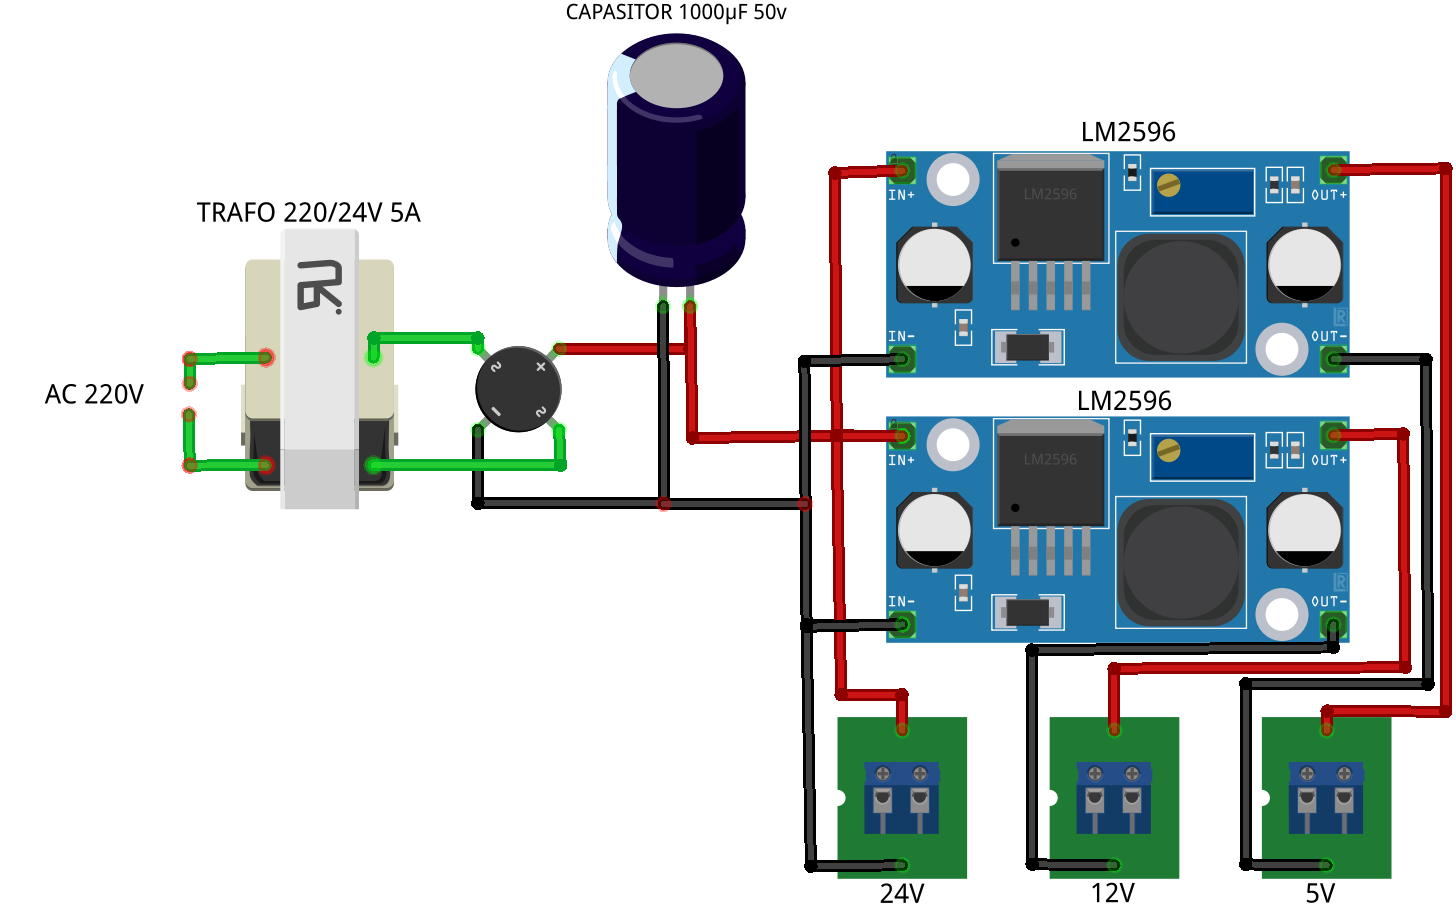
\includegraphics[width=8cm]{gambar/catudaya_bb.png}
	\caption{Trigonometeri Sisi Atas}
	\label{g_ik}
\end{figure}
 
 
Pada robot SCARA, sudut dari \textit{joint} yang dicari merupakan \textit{joint} dari \textit{shoulder} dan juga \textit{elbow.} Kedua \textit{joint} tersebut dapat ditemukan dengan melalui persamaan \textit{pythagoras} dan juga hukum \textit{cosinus}. Pada Gambar 3.17 terlihat bahwa sudut \textit{shoulder} merupakan besar sudut diantara lengan \textit{shoulder} dan juga sumbu x dan sudut elbow merupakan besar sudut antara lengan \textit{elbow} dengan garis bantu dari lengan \textit{shoulder}. Keduanya dapat ditentukan besar nilainya melalui beberapa pesamaan dari \textit{cosinus} dan juga hukum \textit{pyhtagoras}. $l_{1}$ merupakan panjang lengan \textit{shoulder} dan $l_{2}$ merupakan panjang lengan dari \textit{elbow}. Serta $\theta_{1}$ merupakan sudut dari shoulder dan $\theta_{2}$ merupakan sudut dari \textit{elbow}.  

\begin{enumerate}
	\item Dengan menggunakan hukum \textit{cosinus}, didapatkan sebuah persamaan \ref{cosinus1}
	\begin{equation}
	(x^2+y^2)=l_{1}^2+l_{1}^2-2l_{2}l_{2}cos(180-\theta_{2})
	\label{cosinus1}
	\end{equation}
	\item Pada persamaan \ref{cosinus2} terdapat $\cos$ yang dapat diubah sesuai dengan prinsip dari hukum \textit{cosinus} menjadi seperti pada persamaan \ref{cosinus2}
	\begin{equation}
	(x^2+y^2)=l_{1}^2l_{2}^2+2l_{2}l_{2}cos(\theta_{2})
	\label{cosinus2}
	\end{equation}
	\item Pada persamaan \ref{cosinus2} mencari sebuah nilai dari $\theta_{2}$ untuk memmudahkannya maka persamaan menjadi seperti pada persamaan \ref{cosinus3}
	\begin{equation}
	cos(\theta_{2})=\frac{x^2+y^2-l_{1}^2-l_{2}^2}{2_{1}l_{2}}
	\label{cosinus3}
	\end{equation}
	\item Nilai dari $\theta_{2}$ dapat dengan mudah diketahui dengan melanjutkan seperti pada persamaan \ref{cosinus4}
	\begin{equation}
	\theta_{2}=arccos(\frac{x^2+y^2-l_{1}^2-l_{2}^2}{2_{1}l_{2}})
		\label{cosinus4}
	\end{equation}
	Dengan persamaan \ref*{cosinus4} maka nilai dari $\theta_{2}$ atau sudut dari \textit{elbow} dapat diketahui dengan cara memasukkan nilai posisi x, posisi y, serta panjang dari \textit{shoulder} dan \textit{elbow} ke dalam persamaan. Nilai posisi x dan posisi y merupakan posisi akhir dari \textit{end-effector}. 
	\item Dalam menentukan sudut lainnya yaitu sudut \textit{shoulder} yang ditandai dengan simbol $\theta_{1}$ menggunakan persamaan \textit{cosinus} yang dituliskan pada persamaan \ref{cosinus5}
	\begin{equation}
	\frac{sin(\beta)}{l_{2}} = \frac{sin(\gamma)}{\sqrt{x^2+y^2}} ; \alpha=\arctan(\frac{y}{x})
	\label{cosinus5}
	\end{equation}
	\item Pada persamaan \ref{cosinus5} $\sin(\gamma)=\sin(180-\theta_{2})=\sin(\theta_{2})$ dengan mengubah $\sin(\gamma)$ menjadi $\sin(\theta_{2})$ maka akan persamaan menjadi seperi yang ditunjukkan pada persamaan \ref{cosinus6}
	\begin{equation}
	\beta=\arcsin(\frac{l_{2}\sin(\theta_{2})}{\sqrt{x^2+y^2}})
	\label{cosinus6}
	\end{equation}
	\item Jika dilihat pada persamaan \ref{g_ik} makan besar dari sudut \textit{shoulder} yang ditandakan dengan $\theta_{1}$ yang berarti $\theta_{1}=\beta+\alpha$ maka dapat diselesaikan dengan persamaan \ref{cosinus7}
	\begin{equation}
	\theta_{1}=\arcsin(\frac{l_{2}\sin(\theta_{2})}{\sqrt{x^2+y^2}}+\arctan(\frac{y}{x})
	\label{cosinus7}
	\end{equation}
	\item  Dengan penyelesaian seperti pada persamaan \ref{cosinus7} besar sudut dari \textit{shoulder} dapat diketahui dengan memasukkan nilai panjang \textit{elbow}, sudut \textit{elbow} dan juga posisi dari \textit{end-effector}.
\end{enumerate}


